\documentclass[compress]{beamer}
% !TeX document-id = {f19fb972-db1f-447e-9d78-531139c30778}
% !BIB program = biber

%\documentclass[handout]{beamer}
%\documentclass[compress]{beamer}
\usepackage[T1]{fontenc}
\usetheme[block=fill,subsectionpage=progressbar,sectionpage=progressbar]{metropolis} 
\usepackage{graphicx}

\usepackage{wasysym}
\usepackage{etoolbox}
\usepackage[utf8]{inputenc}

\usepackage{pifont}

\usepackage{threeparttable}
\usepackage{subcaption}

\usepackage{tikz-qtree}
\usepackage{neuralnetwork}

\setbeamercovered{still covered={\opaqueness<1->{5}},again covered={\opaqueness<1->{100}}}


\usepackage{listings}

\lstset{
	basicstyle=\scriptsize\ttfamily,
	columns=flexible,
	breaklines=true,
	numbers=left,
	%stepsize=1,
	numberstyle=\tiny,
	backgroundcolor=\color[rgb]{0.85,0.90,1}
}



\lstnewenvironment{lstlistingoutput}{\lstset{basicstyle=\footnotesize\ttfamily,
		columns=flexible,
		breaklines=true,
		numbers=left,
		%stepsize=1,
		numberstyle=\tiny,
		backgroundcolor=\color[rgb]{.7,.7,.7}}}{}


\lstnewenvironment{lstlistingoutputtiny}{\lstset{basicstyle=\tiny\ttfamily,
		columns=flexible,
		breaklines=true,
		numbers=left,
		%stepsize=1,
		numberstyle=\tiny,
		backgroundcolor=\color[rgb]{.7,.7,.7}}}{}


% color-coded listings; replace those above 
\usepackage{xcolor}
\usepackage{minted}
\definecolor{listingbg}{rgb}{0.87,0.93,1}
\setminted[python]{
	frame=none,
	framesep=1mm,
	baselinestretch=1,
	bgcolor=listingbg,
	fontsize=\scriptsize,
	linenos,
	breaklines
	}


\usepackage[american]{babel}
\usepackage{csquotes}
\usepackage[style=apa, backend = biber]{biblatex}
\renewcommand*{\bibfont}{\tiny}


\usepackage{tikz}
\usetikzlibrary{shapes,arrows,matrix}
\usepackage{multicol}

\usepackage{subcaption}

\usepackage{booktabs}
\usepackage{graphicx}



\makeatletter
\setbeamertemplate{headline}{%
	\begin{beamercolorbox}[colsep=1.5pt]{upper separation line head}
	\end{beamercolorbox}
	\begin{beamercolorbox}{section in head/foot}
		\vskip2pt\insertnavigation{\paperwidth}\vskip2pt
	\end{beamercolorbox}%
	\begin{beamercolorbox}[colsep=1.5pt]{lower separation line head}
	\end{beamercolorbox}
}
\makeatother





\setbeamercolor{section in head/foot}{fg=normal text.bg, bg=structure.fg}


\newcommand{\instruction}[1]{\emph{\textcolor{gray}{[#1]}}}



\newcommand{\question}[1]{
	\begin{frame}[plain]
	\begin{columns}
		\column{.3\textwidth}
		\makebox[\columnwidth]{
			\includegraphics[width=\columnwidth,height=\paperheight,keepaspectratio]{mannetje.png}}
		\column{.7\textwidth}
		\large
		\textcolor{orange}{\textbf{\emph{#1}}}
	\end{columns}
\end{frame}}


\tikzstyle{block} = [rectangle, draw, fill=blue!20, 
text width=5em, text centered, rounded corners, minimum height=4em]
\tikzstyle{line} = [draw]
\tikzstyle{pijltje} = [draw, -latex']
\tikzstyle{cloud} = [draw, ellipse,fill=red!20, node distance=3cm,
minimum height=2em, text width=4em, text centered,]


\setbeamercovered{transparent}

\addbibresource{../../resources/literature.bib}
\graphicspath{{../../resources/img/}}


\begin{document}

\title[Big Data and Automated Content Analysis]{\textbf{Big Data and Automated Content Analysis (12EC)} 
\\Week 9: »Transformers«
\\Friday}
\author[Felicia Loecherbach]{Felicia Loecherbach\\ \footnotesize{f.loecherbach@uva.nl \\}}
\date{April 12, 2023}
\institute[UvA CW]{UvA RM Communication Science}


\begin{frame}{}
	\titlepage
\end{frame}

\begin{frame}{Today}
	\tableofcontents
\end{frame}
\begin{frame}[standout]
Before we start: Questions from last week?
\end{frame}


\begin{frame}[standout]
Today: From word embeddings via neural networks towards Transformers
\end{frame}

\question{Remember what we discussed about the move from BOW to word embeddings?}

% deze was eigenlijk voor week 8 gepland, maar zijn we niet aan toegekomen
\section{Neural Networks and Deep Learning}



\subsection[Neural networks]{Neural Networks in Keras}




\begin{frame}{Neural Networks}
	\begin{itemize}
		\item In ``classical'' machine learning, we predict an outcome directly based on the input features
		\item In neural networks, we can have ``hidden layers'' that we predict
		\item These layers are not necessarily interpretable
		\item ``Neurons'' that ``fire'' based on an ``activation function''
	\end{itemize}
	
\end{frame}


\begin{frame}[standout]
Note that in our earlier example with our EmbeddingVectorizer, we essentially added a ``layer'' between the input and the output. Now, we generalize this idea.

\end{frame}

\begin{frame}
	
	\def\layersep{2.5cm}
	
	\begin{tikzpicture}[shorten >=1pt,->,draw=black!50, node distance=\layersep]
	\tikzstyle{every pin edge}=[<-,shorten <=1pt]
	\tikzstyle{neuron}=[circle,fill=black!25,minimum size=17pt,inner sep=0pt]
	\tikzstyle{input neuron}=[neuron, fill=green!50];
	\tikzstyle{output neuron}=[neuron, fill=red!50];
	\tikzstyle{hidden neuron}=[neuron, fill=blue!50];
	\tikzstyle{annot} = [text width=4em, text centered]
	
	% Draw the input layer nodes
	\foreach \name / \y in {1,...,4}
	% This is the same as writing \foreach \name / \y in {1/1,2/2,3/3,4/4}
	\node[input neuron, pin=left:Input \#\y] (I-\name) at (0,-\y) {};
	
	% Draw the hidden layer nodes
	\foreach \name / \y in {1,...,5}
	\path[yshift=0.5cm]
	node[hidden neuron] (H-\name) at (\layersep,-\y cm) {};
	
	
	% Draw the output layer node
	\node[output neuron,pin={[pin edge={->}]right:Output}, right of=H-3] (O) {};
	
	% Connect every node in the input layer with every node in the
	% hidden layer.
	\foreach \source in {1,...,4}
	\foreach \dest in {1,...,5}
	\path (I-\source) edge (H-\dest);
	
	% Connect every node in the hidden layer with the output layer
	\foreach \source in {1,...,5}
	\path (H-\source) edge (O);
	
	% Annotate the layers
	\node[annot,above of=H-1, node distance=1cm] (hl) {Hidden layer};
	\node[annot,left of=hl] {Input layer};
	\node[annot,right of=hl] {Output layer};
	\end{tikzpicture}
	
	$\Rightarrow$ If we had multiple hidden layers in a row, we'd call it a \emph{deep} network.
\end{frame}




\begin{frame}{Why neural networks?}
  \begin{itemize}
  \item learn hidden structures (e.g., embeddings (!))
  \item go beyond the idea that there is a direct relationship between occurrence of word X and label (or occurrence of pixel [R,G,B] and a label)
  \item images, machine translation --- and more and more general NLP, sentiment analysis, etc.
  \end{itemize}
  
  \small {Example of a comparatively easy introduction:
    \url{https://towardsdatascience.com/neural-network-embeddings-explained-4d028e6f0526}}

\end{frame}


\begin{frame}[fragile]{Simple feed forward network}
\begin{lstlisting}
model.add(Dense(300, input_dim=input_dim, activation='relu'))
model.add(Dense(1, activation='sigmoid'))
\end{lstlisting}	
	
\begin{itemize}[<+->]
\item Our first layer reduces the input features (e.g., the 10,000 features our CountVectorizer creates) to 300 neurons
\item It does so using the relu function $f(x) = max(0, x)$ (as our counts cannot be negartive, just a linear function)
\item The second layer reduces the 300 neurons to 1 output neuron using the sigmoid function (the S curve you know from logistic regression)
\item Of course, we can add multiple layers in between if we want to
\end{itemize}
\end{frame}





\begin{frame}{Convolutional networks}
  The problem with such a basic networks: just as with classic SML, we still loose all information about order (the ``not good'' problem).
  Therefore,
  \begin{itemize}
  \item We concatenate the vectors of neighboring words
  \item We apply some filter (essentially, we detect patterns)
  \item and then pool the results (e.g., taking the maximum)
  \end{itemize}
  This means that we now excplitly take into acount \emph{the temporal structure} of a sentence.
\end{frame}



\begin{frame}{Convolutional networks}
  \makebox[\columnwidth]{\includegraphics[width=\columnwidth,height=.8\paperheight,keepaspectratio]{ch09_cnn_cropped}}
\end{frame}

\begin{frame}{Convolutional networks}
	\makebox[\columnwidth]{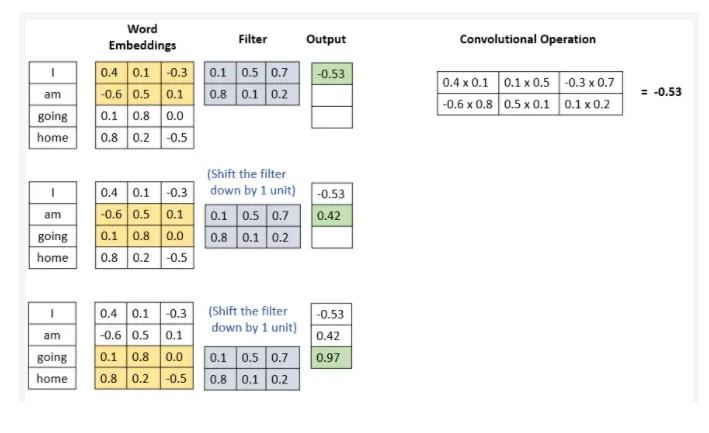
\includegraphics[width=\columnwidth,height=.8\paperheight,keepaspectratio]{cnn_1d.png}}
  \end{frame}



\begin{frame}[fragile]{Convolutional networks}
\begin{lstlisting}
model.add(Embedding(input_dim=vocab_size, output_dim=embedding_dim, input_length=maxlen))
model.add(Conv1D(embedding_dim, 5, activation='relu'))
model.add(GlobalMaxPooling1D())
model.add(Dense(300, activation='relu'))
model.add(Dense(1, activation='sigmoid'))
\end{lstlisting}	
The layers:	
\begin{enumerate}[<+->]
\item train an embedding model
\item apply the convolution with 5 ``timestamps''
\item pool using the maximum
\item another layer with 300 dimensions
\item the final layer with 1 output neuron
\end{enumerate}
\end{frame}


\begin{frame}{Convolutional networks}
  \textbf{Note that the preprocessing differs!}
  
  \begin{itemize}
  \item We do not take a word vector per document as input any more, but \emph{a sequence of words}
  \item For concatenating, these sequences need to have equal length, which is why we \emph{pad} then
  \end{itemize}
	
\end{frame}




\begin{frame}{LSTM (long short-term memory)}
  \begin{itemize}
  \item Unlike ``feed forward'' neural networks, this is  a ``recurrent neural network'' (RNN) -- the training works in two directions
  \item Heavy in computation, very useful for predicting \emph{sequences}
  \item Won't cover today
  \end{itemize}
\end{frame}




\begin{frame}{The embedding layer}
  \begin{itemize}
  \item Often, the first layer is creating word embeddings
  \item Good embeddings need a lot of training data
  \item Training good embeddings needs time
  \item Therefore, we can replace that layer with a pre-trained embedding layer (!)
  \item We can even use a hybrid approach and allow the pre-trained embedding layer to be re-trained!
  \end{itemize}
\end{frame}



\begin{frame}[standout]
  There are example notebooks on github!
\end{frame}


\begin{frame}{Let's look into some code}
\url{https://github.com/uvacw/teaching-bdaca/blob/main/12ec-course/week08/exercises/06downstreamkeras.ipynb}
\end{frame}

\section{Transformers}

\subsection{Some limitations of our approaches so far}

\begin{frame}{Some problems to address}
  Just replacing BOW with word embeddings is not enough:
  \begin{block}{Context}
      \begin{itemize}
      \item ``bank'' (money), ``bank'' (of a river), \ldots $\rightarrow$ all the same word embedding
      \item Understanding references within a sentence (`` who is `she'?'') $\rightarrow$ can actually be done with, for instance, LSTM/RNN
      \end{itemize}
  \end{block}
\end{frame}

\begin{frame}{Some problems to address}
  
  \begin{block}{Tha amount of training data}
      \begin{itemize}
      \item Thousands of annotations needed in traditional BOW
      \item Especially be problematic when we have many and/or small categories
      \item We already argued that pre-trained embeddings can partly mitigate this
      \item Yet, a human doesn't need hundreds of examples but just a few to learn the difference between, say, two animal species (few-shot learning)
      \end{itemize}
  \end{block}
\end{frame}


\begin{frame}{``Attention  is all you need''}
  \begin{itemize}
  \item Title of an extremely influential paper \parencite{Vaswani2017}
  \item Paradigm shift:
  \end{itemize}

 \pause
 \begin{quote}
``The dominant sequence transduction models are based on complex recurrent or
convolutional neural networks that include an encoder and a decoder. The best
performing models also connect the encoder and decoder through an attention
mechanism. We propose a new simple network architecture, the Transformer,
based solely on attention mechanisms, dispensing with recurrence and convolutions
entirely.''
\end{quote}
\end{frame}

\begin{frame}[plain]
  OK, that sounds complicated.
\end{frame}

\begin{frame}{``Attention  is all you need''}
\begin{figure}
	\centering
	\includegraphics[width=.5\linewidth]{transformer_self-attention_visualization.png}
	\caption{The idea of ``attention''. \url{http://jalammar.github.io/illustrated-transformer/}}
	\label{fig:attention}
\end{figure}
\end{frame}


\begin{frame}{The technical details}
  We will not go into all the math behind it -- it's beyond the scope of this class. But there is a nice hands-on explanation of the \textcite{Vaswani2017}-paper including a commented Python implementation available at  \url{http://nlp.seas.harvard.edu/annotated-transformer/}.

  (Further reading if you consider to continue working on this)
\end{frame}


\subsection{BERT, the game changer}

\begin{frame}{Bidirectional Encoder Representations from Transformers}
The famous BERT \parencite{Devlin2018} model

\begin{quote}
`` The
masked language model randomly masks some of
the tokens from the input, and the objective is to
predict the original vocabulary id of the masked word based only on its context. Unlike left-to-
right language model pre-training, the MLM ob-
jective enables the representation to fuse the left
and the right context, which allows us to pre-
train a deep bidirectional Transformer. In addi-
tion to the masked language model, we also use
a “next sentence prediction” task that jointly pre-
trains text-pair representations.''
    \end{quote}

\end{frame}





\begin{frame}{The idea of finetuning}
  \begin{itemize}
  \item BERT (or GPT-4, \ldots) are Large Language Models (LLMs)
  \item Training them is \emph{really} expensive. Training BERT is said to have cost 7,000 USD, GPT-3 even 4,600,000 USD (just for the computing!) 
  \item So, no, you don't do that yourself (nor do universities, normally).
  \item Solution: Separating (unsupervised) pre-training from fine-tuning for downstream tasks!
  \end{itemize}

\end{frame}


\begin{frame}{Pre-training vs fine-tuning}
\begin{figure}
	\centering
	\includegraphics[width=.8\linewidth]{BERT-finetuning.png}
	\caption{Finetuning BERT \parencite{Devlin2018}.}
	\label{fig:finetuning}
\end{figure}

\end{frame}


\begin{frame}{How to fine-tune}
General idea: you download a pre-trained model, than finetune it 
  
  \begin{itemize}
  \item \url{https://www.huggingface.co} is your starting point
  \item We also made an example notebook: \url{https://github.com/uvacw/teaching-bdaca/blob/main/modules/machinelearning-text-exercises/transformers_bert_classification.ipynb}
  \item You probably want to use a GPU (e.g., on Google Colab)
  \end{itemize}

\end{frame}


\begin{frame}{How to fine-tune}
Note that you can fine-tune for very different tasks:
  
  \begin{itemize}
  \item classification ($\rightarrow$ SML)
  \item question answering
  \item translation
  \end{itemize}
\end{frame}


\question{Do you see how this relates to public-facing applications like DALL-E and ChatGPT? Do you see how these relate to encoding, decoding, and transformers?}




\subsection{Critical voices}


\begin{frame}{Stochastic parrots?}
Really read the paper by \parencite{Bender2021}!

Think about:

\begin{itemize}
\item environmental and financial costs
\item bias
\item ethical issues
\item ``amplification of a hegemonic worldview''
\item \ldots
\end{itemize}
  
\end{frame}








\subsection{Practical example}


\begin{frame}{\textcite{Lin2023}}

  Can we train a model to rate news items \emph{from very different sources such as newspaper articles, videos, podcasts, blogs, \ldots } on two scales
  \begin{enumerate}
  \item informal --- formal
  \item factual --- opinionated
  \end{enumerate}
to identify/describe their genre?
\end{frame}


\begin{frame}[plain]
\begin{figure}
	\centering
	\includegraphics[width=\linewidth]{lin2013-1.png}
\end{figure}
\end{frame}


\begin{frame}[plain]
\begin{figure}
	\centering
	\includegraphics[width=\linewidth]{lin2013-2.png}
\end{figure}
\end{frame}


\begin{frame}[plain]
\begin{figure}
	\centering
	\includegraphics[width=\linewidth]{lin2013-3.png}
\end{figure}
\end{frame}


\begin{frame}{\textcite{Lin2023}}
  \begin{itemize}
  \item BOW approaches cannot achieve this well enough, but finetuning a transformer can improve the classification
  \item They can generalize across \emph{very} different formats
  \end{itemize}

\end{frame}





\begin{frame}{Finally: Some links}
\begin{itemize}
\item \url{https://nlp.seas.harvard.edu/2018/04/03/attention.html}
\item \url{http://jalammar.github.io/illustrated-transformer/}
\end{itemize}
\end{frame}






\begin{frame}[standout]
Let's look into Google Colab!
\end{frame}


\section{Next steps}
\begin{frame}[standout]
Try it yourself!
\url{https://github.com/uvacw/teaching-bdaca/blob/main/12ec-course/week09/exercises/README.md}
\end{frame}


\begin{frame}[allowframebreaks,plain]
\printbibliography
\end{frame}



\end{document}
